% Sample LaTeX file for creating a paper in the Morgan Kaufmannn two
% column, 8 1/2 by 11 inch proceedings format.
\documentclass{article}
\usepackage{proceed2e}
\usepackage[margin=1in]{geometry}
% Set the typeface to Times Roman
\usepackage{times}
\usepackage{amsmath}
\usepackage{amssymb}
\usepackage{bbm}
\usepackage{graphics}
\usepackage{graphicx}
\usepackage{booktabs}
%\usepackage[demo]{graphicx}
\usepackage{caption}
\usepackage{subcaption}
\usepackage{color}
\usepackage{algorithm}
\usepackage{algorithmic}
\usepackage[round, comma, sort]{natbib}

%\title{Maximum Entropy Clustering Counting in Large Social Graphs}
\title{Entropic Spectral Learning in Large Scale Networks}
\newtheorem{proposition}{Proposition}
%\author{} % LEAVE BLANK FOR ORIGINAL SUBMISSION.
% UAI  reviewing is double-blind.
% The author names and affiliations should appear only in the accepted paper.
%
%\author{ {\bf Harry Q.~Bovik\thanks{Footnote for author to give an
%alternate address.}} \\
%Computer Science Dept. \\
%Cranberry University\\
%Pittsburgh, PA 15213 \\
%\And
%{\bf Coauthor}  \\
%Affiliation          \\
%Address \\
%\And
%{\bf Coauthor}   \\
%Affiliation \\
%Address    \\
%(if needed)\\
%}
\begin{document}

\maketitle

\begin{abstract}
We present a novel algorithm for learning the spectral density of large scale networks using stochastic trace estimation and maximum entropy method. The algorithms complexity is linear in the number of non-zeros of the matrix which is a great computational advantage when compared to other algorithms. We apply our algorithm to the problem of community detection in large networks and to determining the similarity between different networks using the Jensen Shannon divergence. We show state-of-the-art performance on both synthetic and real datasets against compareable methods. 
\end{abstract}

%%%%%%%%%%%%%%%%%%%%%%%%%%%%%%%%%%%%%%%%%%%%%%%%%%%%%%%
%%%%%%%%%%%%%%%%%%   Introduction  %%%%%%%%%%%%%%%%%%%%%%
%%%%%%%%%%%%%%%%%%%%%%%%%%%%%%%%%%%%%%%%%%%%%%%%%%%%%%%

\section{INTRODUCTION}

\subsection{The Importance of Networks}
Many systems of interest, can be naturally characterised by complex networks; examples include social networks \citep{{mislove2007measurement},{flake2000efficient},{leskovec2007dynamics}}, biological networks \citep{palla2005uncovering} and technological networks. The biological cell, can be compactly described as a complex network of chemical reactions; trends, opinions and ideologies spread on a social network, in which people are nodes and edges represent relationships, the world wide web is a complex network of documents (web pages representing nodes) with hyper-links denoting edges. A variety of complex graphs have been studied, from scientific collaborations, ecological/cellular networks, to sexual contacts \citep{albert2002statistical}. For a comprehensive introduction, we recommend the work by \citet{newman2010networks} .

\subsection{Communities and their Importance}
One of the most important research questions in network analysis is community detection \citep{fortunato2010community}.
In protein-protein interaction networks, communities are likely to group proteins having the same cellular function \citep{chen2006detecting}. In the world wide web, communities may correspond to pages dealing with related topics \citep{dourisboure2007extraction}. In social networks, they may correspond to families, friendship circles, towns and nations. 

Communities also have concrete practical applications. Clustering geographically close web users with similar interests could improve web performance by serving them with a dedicated mirror server \citep{krishnamurthy2000network}. Identifying clusters of customers with similar purchasing interests allows for the creation of efficient reccomender systems \citep{reddy2002graph}. For a full review of the importance of clustering and various methods in the literature, we recommend the work by \citet{fortunato2010community}.

%%%%%%%%%%%%%%%%%%%%%%%%%%%%%%%%%%%%%%%%%%%%%%%%%%%%%%%
%%%%%%%%%%%%%%%%%%   Motivating Example  %%%%%%%%%%%%%%%%%%%%%%
%%%%%%%%%%%%%%%%%%%%%%%%%%%%%%%%%%%%%%%%%%%%%%%%%%%%%%%

\section{MOTIVATING EXAMPLE }
In the fields of statistics, computer science and machine learning, spectral clustering \citep{von2007tutorial} has become an incredibly powerful tool for grouping data, regularly outperforming or enhancing other classical algorithms, such as $k$-means or single linkage clustering.

For most clustering algorithms, estimating the number of clusters is an open problem \citep{von2007tutorial}, with likelihood, ad-hoc, information theoretic, stability and spectral approaches advocated. In the latter, one analyses the spectral gap in the eigenvalue spectrum which we refer to as eigengap for short. Applying this approach in the era of big-data (where social networks such as Facebook are approaching $2$ billion users) means that standard approaches, such as the canonical Cholesky decomposition, with computational complexity $\mathcal{O}(n^{3})$  and storage $\mathcal{O}(n^{2})$ are completely prohibitive. 


We propose a novel maximum entropy algorithm, which we use along with Chebyshev stochastic trace estimation to learn the spectral density of a network. This entails computational complexity $\mathcal{O}(n_\mathrm{nz})$,  where $n_\mathrm{nz}$ represents the number of non-zeros elements of the matrix. For a network such as Facebook, where the average user has $300$ friends, this potentially represents a speedup of up to $\mathcal{O}(10^{16})$.

We prove a bound on the positive deviation from zero using matrix perturbation theory and the Cauchy-Schwarz inequality for weakly connected clusters and demonstrate its effectiveness on synthetic examples. Having learned the spectrum, we search for a spectral minimum near the origin\footnote{Corresponding to the eigengap.} and determine the number of clusters. We test our algorithm on both synthetic and real data with available ground truth and show superior performance to the state-of-the-art iterative method. We further provide analytical formulae for the network differential entropy and divergence between networks, which have been used to quantify graph stfucture and similarity respectively \citep{takahashi2012discriminating}.

\subsection{Related Work} 
Krylov subspace methods, using matrix vector products, such as the Lanczos algorithm have been applied to estimating eigengaps and to detect communities with encouraging results \citep{{ubaru2017fast},{kang2011spectral}}.
The computational complexity of the Lanczos algorithm is $\mathcal{O}(n_\mathrm{nz}\times m_s + nm_s^{2})\times d$, where $n$ is the rank of the square matrix $M \in \mathbb{R}^{n\times n}$,
$d$ the number of random starting vectors used and $m_s$ the number of Lanczos steps taken. 
The computational complexity of our Entropic Spectral Learning is $\mathcal{O}(n_\mathrm{nz}\times m)\times d$, where $m$ is the number of moments used, as there is no need to orthogonalise the Lanczos vectors at each step. The second Lanczos term dominates at $m_s > n_\mathrm{nz}/n$. For many networks in the Stanford Large Network Dataset Collection (SNAP)\citep{snapnets}, such as Amazon, YouTube, Wikipedia and LiveJournal, this condition is reached for low values of $m_s = [3,3,14,6]$ respectively. We find empirically that for good spectral resolution $m_s>50$, the extra computational overhead for Lanczos is substantial. We compare our method against Lanczos algorithm on both synthetic and real datasets and our method shows superior performance.

%%%%%%%%%%%%%%%%%%%%%%%%%%%%%%%%%%%%%%%%%%%%%%%%%%%%%%%
%%%%%%%%%%%%%%%%%%   Graph Notation  %%%%%%%%%%%%%%%%%%%%%%
%%%%%%%%%%%%%%%%%%%%%%%%%%%%%%%%%%%%%%%%%%%%%%%%%%%%%%%

\section{GRAPH NOTATION }
Graphs are the mathematical structure underpinning the formulation of networks. Let $G = (V,E)$ be an undirected graph with vertex set $V = {v_{1},...v_{N}}$. Each edge between two vertices $v_{i}$ and $v_{j}$ carries a non-negative weight $w_{ij}>0$ and $w_{ij}=0$ corresponds to two disconnected nodes. For un-weighted graphs we set $w_{ij}=1$ for two connected nodes. The \textbf{adjacency matrix} is defined as $W = (w_{ij})$ with $i,j=1,...n$. The degree of a vertex $v_{i} \in V$ is defined as 
\begin{equation}
d_{i} = \sum_{j=1}^{n}w_{ij}.
\end{equation}
The \textbf{degree matrix} $D$ is defined as a diagonal matrix that contains the degrees of the vertices along diagonal, i.e., $D_{ii} = d_{i}$. The \textbf{unnormalised graph Laplacian matrix} is defined as
\begin{equation}
L = D - W.
\end{equation}
As $G$ is undirected $w_{ij}=w_{ji}$, which means that the weight matrix is symmetric and hence $W$ is symmetric. Since every diagonal matrix is symmetric, the unnormalised Laplacian matrix is also symmetric. This ensures that the eigenvalues of the Laplacian are real. Another common characterisation of the Laplacian matrix is the \textbf{Normalised Laplacian matrix} \citep{chung1997spectral}
\begin{eqnarray}
L_{\mathrm{norm}} &=& D^{-1/2}LD^{-1/2}  \nonumber\\
 &=& I - \tilde{W} = I - D^{-1/2}WD^{-1/2}\label{lnorm}
\end{eqnarray}
where $\tilde{W}$ is known as the normalised adjacency matrix\footnote{Strictly speaking, the second equality only holds for graphs without isolated vertices.}. For our analysis we will be using the Laplacian matrix. 
There is no commonly adopted convention on which Laplacian to use. For regular graphs, where most vertices have the same degree, all Laplacians are similar to each other \citep{von2007tutorial}, but outside this regime, they vary considerably. For our experiments, we use the normalised Laplacian but we could have just as well used the unnormalised Laplacian and divided by the Gershgorin bound \citep{gershgorin1931uber} or the number of nodes $n$.

%%%%%%%%%%%%%%%%%%%%%%%%%%%%%%%%%%%%%%%%%%%%%%%%%%%%%%%
%%%%%%%%%%%%%%%%%%   Graph Eigenstructure  %%%%%%%%%%%%%%%%%%%%%%
%%%%%%%%%%%%%%%%%%%%%%%%%%%%%%%%%%%%%%%%%%%%%%%%%%%%%%%

\section{GRAPH EIGENSTRUCTURE}
Isomorphic graphs are co-spectral. This means that any relabelling of node numbers has no effect on their adjacency matrices after a permutation of rows and columns. Spectral techniques have been used extensively to characterise global network structure \citep{newman2006modularity} and in practical applications thereof, such as facial recognition/computer vision \citep{belkin2003laplacian} and to learn dynamical thresholds \citep{mcgraw2008laplacian}.
\\
 \includegraphics[width=0.5\textwidth]{saltire}
Whilst there exist non-isomorphic cospectral graphs, such as the Saltire pair shown above, computer simulations show that beyond $n\geq9$ vertices, the fraction $f$ of graphs with cospectral adjacency and Laplacian matrices decreases and it is conjectured that for $n\rightarrow\infty$ that $f\rightarrow 0$. Furthermore the spectrum of the adjacency and the Laplacian matrices can be used to deduce important quantities, such as the number of vertices/edges, where the graph is regular (fixed girth) / bipartite, the number of closed walks, the number of components and the number of spanning trees \citep{van2003graphs}.


%%%%%%%%%%%%%%%%%%%%%%%%%%%%%%%%%%%%%%%%%%%%%%%%%%%%%%%
%%%%%%%%%%%%%%  Clustering using  Eigenspectra  %%%%%%%%%%%%%%%%%%%%%%
%%%%%%%%%%%%%%%%%%%%%%%%%%%%%%%%%%%%%%%%%%%%%%%%%%%%%%%


\section{CLUSTERING USING THE EIGENSPECTRA}
We reproduce the well-known result that the number of zero eigenvalues of the graph $G$ indicates the number of connected components. We then use matrix perturbation theory and the Cauchy-Schwarz inequality to show that by adding a small amount of edges between the connected components, these eigenvalues are perturbed by a small positive amount. Hence if this perturbation is small compared to the original spectral gap, we can still determine the number of clusters by integrating the spectral density until the first minimum and then multiplying by the dimension of the Laplacian matrix.
\begin{proposition}
	\label{numberof0eigenvalues}
	Let G be an undirected graph with non-negative weights. Then the multiplicity $k$ of the eigenvalue $0$ of the Laplacian $L\in \mathcal{R}^{n\times n}$ is equal to the number of connected components $A_{1},...A_{k}$ in the graph. The eigenspace of the eigenvalue $0$ is spanned by the indicator vectors $\mathbbm{1}_{A_{1}},....\mathbbm{1}_{A_{k}}$
	\end{proposition} 
An intuitive proof can be found in \citep{von2007tutorial}, which we outline for completeness. Note that by the definition of the unnormalised Laplacian, that $L_{ij} = \mathbbm{1}_{i=j}\sum_{k=1}^{n}w_{ik}-w_{ij}$ and hence for $u_{j} = 1$
\begin{equation}
u_{i} = \sum_{j=1}L_{ij}u_{j} = \sum_{j=1}\bigg(\mathbbm{1}_{i=j}\sum_{k=1}w_{ik} - w_{ij}\bigg) = 0 
\end{equation}
This proves that the vector $u = [1,....,1]^T$ is an eigenvector with eigenvalue $0$. For $k$ connected components, the matrix $L$ has block diagonal form
\[
\begin{bmatrix}
	L_{1} & \dots  & \dots \\
	\dots & \ddots & \dots  \\
	\dots & \dots & L_{k}
\end{bmatrix}
\]
As is the case for all block diagonal matrices, the spectrum of $L$ is given by the union of the spectra $L_{i}$. From the proceeding we know that every Laplacian $L_{i}$ has an eigenvalue $0$ with multipicity $1$, hence $L$ has eigenvalue $0$ with multiplicity $k$ and corresponding eigenvectors of $L$ are those of $L_{i}$ filled with $0$ at the positions of the other blocks. 

Hence to learn the number of disconnected components in an arbitary graph, we simply count the number of $0$ eigenvalues. However given that real world networks are rarely completely disconnected, this procedure would be of little practical utility. 


We hence consider a looser definition of the word cluster and consider groups of nodes containing far greater intra-group connections than inter-group connections. This conforms to our natural intuition of a group or community.  

If the graph is connected, but consists of $k$ subgraphs which are ``weakly'' linked to each other, the unnormalized Laplacian will have one zero eigenvalue and all the other eigenvalues positive. This is easily seen by looking at
\begin{equation}
u^{t}Lu = \sum_{i,j=1}^{n}w_{ij}(u_{i}-u_{j})^{2}
\end{equation}
which is positive semi-definite, as $w_{ij}>0$ and we have proved that a connected graph $G$ has one $0$ eigenvalue, hence all other eigenvalues are positive. For small changes in the Laplacian, we expect from matrix perturbation theory \citep{bhatia2013matrix} that the next $k-1$ smallest eigenvalues to be close to $0$. If we consider a small perturbation of the Laplacian $\tilde{L} = L +\delta L$, where $|| \delta L|| \ll ||L||$, then it can be shown that $\forall \thinspace 1\leq i\leq k $, the difference in the $i$-th eigenvalue can be written as 
\begin{equation}
\label{cauchyschwarz}
\lambda_{i}' - \lambda_{i} = u_{i}^{t}\delta L u_{i} \leq ||\delta L||\thinspace||u_{i}^{t}u_{i}|| = ||\delta L||
\end{equation}
where we have used the orthonormality of the eigenvectors, the eigenvalues of the unperturbed matrix and the Cauchy Schwarz inequality. 

If we consider the natural variant of the Laplacian, normalised by the number of vertices in the graph, i.e $L_\mathrm{natural} = (D-A)/n$, then by adding $R$ vertices between previously disconnected subgraphs, for each vertex, we alter a two diagonal components by $+1$ and two off diagonal components by $-1$.Thus, our bound goes as $R/n$ by using the Frobenius norm . We note that our derived bound using the Cauchy Schwarz inequality is exactly the same as Weyl's perturbation theorem for Hermitian matrices, which uses the min-max principle \citep{bhatia2013matrix}.


Hence we expect the eigenvalue perturbations to die off as $\mathcal{O}(n^{-1})$ for a constant number of connections between clusters as we increase the number of nodes $n$ in the network. Even if the number of such connections grows with $n$ but is sparse such that the total number is $\mathcal{O}(n s)$ with small sparsity $s$, the perturbation would only be of order $s$ and for small sparsity $s$ we would expect our algorithm to also work in those cases.

\begin{figure}[t]
	\begin{subfigure}{.32\linewidth}
		\centering
		\includegraphics[trim=0.1cm 0.1cm 1cm  1cm, clip, width=1.0\linewidth]{10erdosrenyip1}
		\caption{}
		\label{fig:sub1}
	\end{subfigure}
	\begin{subfigure}{.32\linewidth}
		\centering
		\includegraphics[trim=0.1cm 0.1cm 1cm  1cm, clip, width=1.0\linewidth]{3erdosclusters}
		\caption{}
		\label{fig:sub2}
	\end{subfigure}
	\begin{subfigure}{.32\linewidth}
		\centering
		\includegraphics[trim=0.1cm 0.1cm 1cm  1cm, clip, width=1.0\linewidth]{3strogatzclusters}
		\caption{}
		\label{fig:sub3}
	\end{subfigure}
	\caption{(a) Erdos-Renyi random graph with $p=0.1$ and $n=10$ nodes; (b) 3 Watz-Strogatz clusters with $p=0.1,k=5,n=10$ where each cluster is connected by a single node; (c) Watz-Strogatz with $p=0.2$, $k=5$ \& $n=10$ }
	\label{fig:test}
\end{figure}


If we choose to work with the normalised Laplacian \eqref{lnorm}, then for each new connection between previously disconnected components we get a term of the form
%\begin{equation}
\begin{align}
 & \sum_{j=1}\bigg|\bigg|\frac{1}{\sqrt{d_{i}d_{j}}}-\frac{1}{\sqrt{(d_{i}+1)d_{j}}}\bigg|\bigg|^{2}+\frac{2}{(d_{i}+1)(d_{k+1})} \nonumber \\
 & + \sum_{l=1}\bigg|\bigg|\frac{1}{\sqrt{d_{k}d_{l}}}-\frac{1}{\sqrt{(d_{k}+1)d_{l}}}\bigg|\bigg|^{2}
 \end{align}
%\end{equation}
where nodes $k$ and $i$ are being connected and nodes $j$ and $l$ are the nodes connected to $k$ and $i$, respectively. By taking the degrees to be a fraction of the total number of nodes $n$ and taking $n$ to be large we observed a similar $n^{-1}$ scaling. The idea of strong communities being nearly disconnected components, is not novel \citep{mcgraw2008laplacian} and has been used in community detection algorithms \citep{capocci2005detecting}. However we have not come across a simple exposition of the results from matrix perturbation theory, or the application of the Cauchy Schwarz inequality to bound the increase in the $0$ eigenvalues as a function of node number $n$ or degrees $d_{i}$ amongst the connected components.


	%\caption{A figure with two subfigures}

\begin{table}[t]
	\caption{Second and Third smallest eigenvalues of 3 initially disconnected sets of connected nodes of size $n$ connected by a single inter-node link}\label{table1}
	\begin{center}
		\begin{small}
			\begin{sc}
				\begin{tabular}{lcccr}
					\toprule
					$n$ & Erdos-Renyi & Watts-Strogatz  \\
					& ($p=1$) & $(p=0.3,k=5$)  \\
					\midrule
					$10^{1}$    & [$8\times 10^{-2},2\times 10^{-1}$]& [$6\times 10^{-2},2\times 10^{-1}$]  \\
					$10^{2}$ & [$9\times 10^{-3},2\times 10^{-2}$]& [$4\times 10^{-3},1\times 10^{-2}$]\\
					$10^{3}$    & [$9\times 10^{-4},3\times 10^{-3}$]& [$6\times 10^{-4},1\times 10^{-3}$] \\
					\bottomrule
				\end{tabular}
			\end{sc}
		\end{small}
	\end{center}
	\vskip -0.1in
\end{table}



\begin{table}[t]
\caption{Second and Third smallest eigenvalues of 3 initially disconnected sets of connected nodes of size $n$ connected by a number of links $R=0.1n$ proportional to the number of nodes}	\label{table2}
	\begin{center}
		\begin{small}
			\begin{sc}
				\begin{tabular}{lcccr}
					\toprule
					$n$ & Erdos-Renyi  & Watts-Strogatz  \\
					& ($p=0.3$) & $(p=0.1,k=5$)  \\
					\midrule
					$10^{1}$    & [$1\times 10^{-1},2\times 10^{-1}$]& [$2\times 10^{-1},2\times 10^{-1}$]  \\
					$10^{2}$ & [$2\times 10^{-1},2\times 10^{-1}$]& [$2\times 10^{-2},5\times 10^{-2}$]\\
					$10^{3}$    & [$3\times 10^{-1},3\times 10^{-1}$]& [$2\times 10^{-2},3\times 10^{-2}$] \\
					\bottomrule
				\end{tabular}
			\end{sc}
		\end{small}
	\end{center}
	\vskip -0.1in
\end{table}

We test the intuition derived by this bound by generating $k$ connected traditional random graphs of equal size and forming the disjoint union.  The number of $0$ eigenvalues is given by Proposition \ref{numberof0eigenvalues}, which we verify to within numerical precision. We then create a number of links between the clusters and see how the next $k-1$ smallest non-zero eigenvalues change in size. The results for Erdos-Renyi \citep{erdos1959random} and Watts-Strogatz \citep{watts1998collective} random graphs of different sizes and parameter values are shown in Tables \ref{table1} and \ref{table2}. We see that for a constant number of connections between the clusters, \ref{table1}, in this case one interconnected node between the clusters, the smallest non-zero eigenvalues are peturbed from $0$ to $n^{-1}$ as expected from our bound. In Table \ref{table2}, where we create a number of inter-nodal links proportional to the number of nodes\footnote{Or alternatively cluster members.}, with the exception of the very small Strogatz network, we have eigenvalues of similar order. We also test for sizes $n=500$ and $n=2000$ and find that the Eigenvalues stay of similar size to the other values in the table.


Hence, the number of communities can be approximated as the number of small eigenvalues close to 0. For a continous spectral density this can be written as 
\begin{equation}
C = n\int_{0}^{\lambda*} p(\lambda)d\lambda
\end{equation}
with $n$ being the number of nodes and $\lambda*$ being the location of the first spectral minimum corresponding to the spectral gap. 

As a final remark, note that in the context of the above discussed random graph models, the Laplacian will be a random matrix. There are powerful techniques from random matrix theory which provide analytical expressions for eigenvalue densities of such random matrices (see \cite{RMTbook} for an overview). 

%Hence, in the event that they exist, to detect the number of densely connected clusters, or communities with much stronger intra community than inter community connections, we search for a spectral gap near the origin. Given the spectral density we integrate until the spectral minimum and multiply by the size of the matrix.....  

\begin{figure}[t]
	\centering
	\includegraphics[trim=1.0cm 0.5cm 0.5cm  0.5cm, clip, width=1.0\linewidth]{3erdosclusters}
	\caption{3 Watts-Strogatz clusters with $p=0.1,k=5,n=10$ where each cluster is connected by a single node. }
	\label{fig:sub3}	
\end{figure}

%%%%%%%%%%%%%%%%%%%%%%%%%%%%%%%%%%%%%%%%%%%%%%%%%%%%%%%
%%%%%%%  Estimating the Spectral Density using Maximum Entropy  %%%%%%%%%%%
%%%%%%%%%%%%%%%%%%%%%%%%%%%%%%%%%%%%%%%%%%%%%%%%%%%%%%%


\section{ESTIMATING THE SPECTRAL DENSITY USING MAXIMUM ENTROPY}
\label{maxent}
The method of maximum entropy, hereafter referred to as MaxEnt \citep{Presse2013} is a procedure for generating the most conservative estimate\footnote{With respect to the uniform distribution.} of a probability distribution possible with the given information, the most non-committal with regard to missing information \citep{Jaynes1957}.

To determine the spectral density $p(\lambda)$, we maximise the entropic functional 
\begin{equation}
\label{BSG}
S = - \int p(\lambda)\log p(\lambda)d\lambda- \sum_{i}\alpha_{i}\bigg[\int p(\lambda)\lambda^{i}d\lambda - \mu_{i}\bigg]
\end{equation}
with respect to $p(\lambda)$, where $ \mathbb{E}[ \lambda^{i}]= \mu_{i}$ are the power moment constraints on the spectral density, which are estimated using stochastic trace estimation. 

The first term in equation \eqref{BSG} is referred to as the Boltzmann-Shannon-Gibbs (BSG) entropy, which has been applied in multiple fields, ranging from condensed matter physics~\citep{Giffin2016} to finance~\citep{Neri2012,Buchen1996}.
Under the axioms of consistency, uniqueness, invariance under coordinate transformations, sub-set and system independence, it can be proved that for constraints in the form of expected values, drawing self-consistent inferences requires maximising the entropy \citep{{Shore1980},{Presse2013}}.


\subsection{Stochastic Trace Estimation}
Using the expectation of quadratic forms, for any multivariate random variable $v$ with mean $m_z$ and variance $\Sigma$, we can write 
\begin{equation}
\mathbb{E}(zz^{t}) = m_z m_z^{t}+\Sigma \xrightarrow[m_z = 0]{\Sigma = I} I,
\end{equation}
where in the last relation we have assumed that the variable possesses zero mean and unit variance. By the linearity of trace and expectation for any $m_z \geq 0$
\begin{equation}
\sum_{i=1}^{n}\lambda_{i}^{m_z} = n\mathbb{E}_{\mu}(\lambda^{m_z}) = \text{Tr}(IK^{m_z}) = \mathbb{E}(zK^{m_z}z^{t}).
\end{equation}
We approximate the expectation over all random vectors with a simple Monte Carlo average. i.e for $d$ random vectors ,
\begin{equation}
\mathbb{E}(zK^{m_z}z^{t}) \approx \frac{1}{d}\bigg(\sum_{j=1}^{d}z_{j}K^{m_z}z_{j}^{t} \bigg),
\end{equation}
where we take the product of the matrix $K$ with the vector $z_{j}$, $m$ times, so as to avoid costly $\mathcal{O}(n^{3})$ matrix matrix multiplication. This allows us to calculate the non central moment expectations in $\mathcal{O}(dm\times n_\mathrm{nz})$ for sparse matrices, where $d\times m \ll n$.

The random unit vector $z_{j}$ can be drawn from any distribution, such as a Gaussian. Choosing the components of $z_{j}$ to be i.i.d Rademacher random variables i.e $P(+1)=P(-1) = \frac{1}{2}$ via Hutchinson's method \citep{hutchinson1990stochastic} has the lowest variance of such estimators.
Loose bounds exist on the number of samples $d$ required to get within a fractional error $\epsilon$ with probability close to one \citep{han2015large}.

\subsection{Analytical forms for the Differential Entropy and Divergence from MaxEnt}
In other work using either the exact eigen-decomposition \citep{takahashi2012discriminating} or Chebyshev/Lanczos \citep{ubaruapplications} as the differential entropy of delta function
\begin{equation}
\mathcal{S}(\delta(x)) = 1/2 \log(2\pi e\sigma^{2}) \xrightarrow{\sigma\rightarrow 0} -\infty .
\end{equation}
Gaussian Kernel regression, along with a prescriptions for the Bandwidth using the Sturges criterion is used. Given that neither the differential entropy of a Gaussian mixture nor the Kullback-Leiber/Shannon-Jensen divergence between a Gaussian mixture has an analytical form \citep{hershey2007approximating}, this too must be approximated using either Monte-Carlo sampling or numerical quadrature. An advantage of the Maximum Entropy formalism is that both can be calculated trivially after having completed the optimisation.
To calculate the differential entropy we simply note that
\begin{equation}
\mathcal{S}(p) = \int p(\lambda) (1+\sum_{i}^{m}\alpha_{i}x^{i}) d\lambda= 1+\sum_{i}^{m}\alpha_{i}\mu_{i}
\end{equation}
where $p(\lambda) = \exp[-(1+\sum_{i}^{m}\alpha_{i}x^{i})]$.


The KL divergence between two Maximum Entropy spectra, $p(\lambda) = \exp[-(1+\sum_{i}\alpha_{i}x^{i})]$ and $q(\lambda) = \exp[-(1+\sum_{i}\beta_{i}x^{i})]$, can be written as
\begin{equation}
\mathcal{D}_{kl}(p||q) = \int p(\lambda)\frac{p(\lambda)}{q(\lambda)}d\lambda = -\sum_{i}(\alpha_{i}-\beta_{i})\mu_{p}^{i},
\end{equation}
where $\mu_{p}^{i}$ refers to the $i$-th moment constraint of the density $p(\lambda)$. Similarly the Jensen-Shannon divergence can be written as 
\begin{equation}
\frac{\mathcal{D}_{kl}(p||q)+\mathcal{D}_{kl}(q||p)}{2} = \frac{\sum_{i}(\alpha_{i}-\beta_{i})(\mu_{q}^{i}-\mu_{p}^{i})}{2},
\end{equation}
where all the $\alpha_{i}$ and $\beta_{i}$ are derived from the optimisation and the $\mu$'s are given from the stochastic trace estimation.

%%%%%%%%%%%%%%%%%%%%%%%%%%%%%%%%%%%%%%%%%%%%%%%%%%%%%%%
%%%%%%%%%%%%%%%%%%%  EXPERIMENTS  %%%%%%%%%%%%%%%%%%%%%%%
%%%%%%%%%%%%%%%%%%%%%%%%%%%%%%%%%%%%%%%%%%%%%%%%%%%%%%%

\section{EXPERIMENTS}
We use $d=100$ Gaussian random vectors for our stochastic trace estimation, for both MaxEnt and Lanczos \citep{ubaru2017fast}. When comparing MaxEnt with Lanczos we set the number of moments $m$ equal to the number of Lanczos steps $m_s$ i.e. $m = m_s$. We implement a quaderature MaxEnt algorithm \ref{alg:maxent}. We use a grid size of $10^{-4}$ over the interval $[0,1]$ and add diagonal noise on the Hessian to improve conditioning. We further use Chebyshev polynomial input instead of power moments for improved performance and conditioning. In order to normalise the moment input we use the normalised Laplacian with eigenvalues bounded by $[0,2]$ and divide by $2$. We use Python's in-built optimiser for both the MaxEnt lagrange multipliers and the parameters of the random networks of minimum divergence to our objective. 
\begin{algorithm}[tb]
	\caption{MaxEnt Algorithm}
	\label{alg:maxent}
	
	\begin{algorithmic}[1]
		\STATE {\bfseries Input:} Moments $\{\mu_{i}\}$, Tolerance $\epsilon$, Hessian noise $\eta$
		\STATE {\bfseries Output:} Coefficients $\{\alpha_{i}\}$
		\STATE Initialize $\alpha_{i} = 0$.
		\STATE Minimize $\int_{0}^{1}p_{\alpha}(\lambda)d\lambda + \sum_{i}\alpha_{i}\mu_{i}$
		\STATE Gradient $\mu_{j}-\int_{0}^{1}q_{\alpha}(\lambda)\lambda^{j}d\lambda$
		\STATE Hessian  $ = \int_{0}^{1}p_{\alpha}(\lambda)\lambda^{j+k}d\lambda$
		\STATE Hessian $= (H+H')/2 + \eta$
		\STATE Until $\forall j$ Gradient$_{j} < \epsilon$		
		%\UNTIL{$noChange$ is $true$}
	\end{algorithmic}
\end{algorithm}


\subsection{Synthetic Data}
In order to test the robustness of the approach to networks with clusters of different structures, we implement a mixture of Erdos-Renyi, Watts-Strogatz and Barabási-Albert networks using the Python package \textit{NetworkX} and conduct multiple experiments using networks that have from $3$ to $60$ clusters, with each cluster containing $30$ nodes. We connect the nodes between clusters randomly, with a single inter-cluster connection. 

We display the results for $30$ clusters in Figure \ref{fig:sub3} and $60$ clusters in Figure \ref{fig:sub4}. We see that for an equivalent number of matrix vector calculations, MaxEnt outperforms the Lanczos algorithm. As there is no accepted prescription by which we can determine when the spectral minimum has been best learned, the occasional dips in error produced by Lanczos (such as for $15$ moments in Figure \ref{fig:sub3} are unlikely to be replicated in real world experiments.
\begin{figure}[t]
	\centering
	\begin{subfigure}{.5\linewidth}
		\centering
		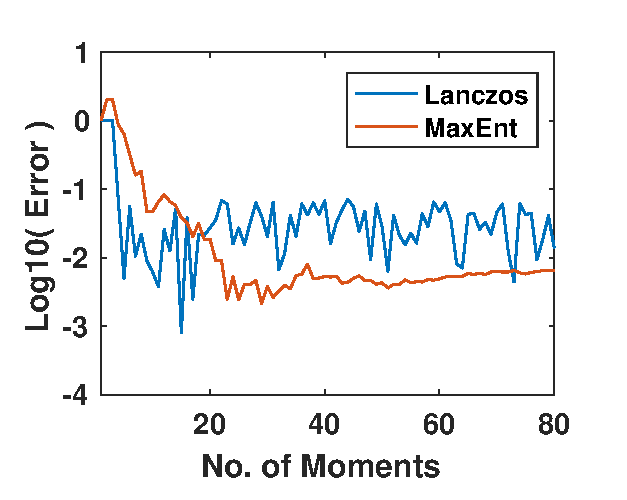
\includegraphics[trim=0.5cm 0.2cm 1cm 0.8cm, clip, width=1.0\linewidth]{Figures/Error_for_Synall3type_connected30}
		\caption{$30$ connected Clusters}
		\label{fig:sub3}
	\end{subfigure}%
	\begin{subfigure}{.5\linewidth}
		\centering
		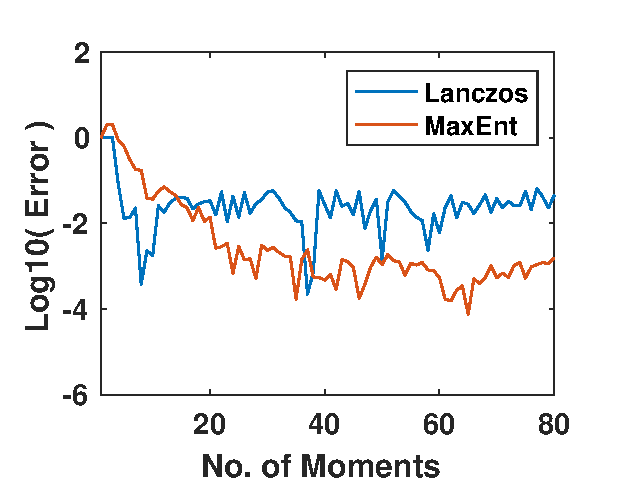
\includegraphics[trim=0.5cm 0.2cm 1cm 0.8cm, clip, width=1.0\linewidth]{Figures/Error_for_Synall3type_connected60}
		\caption{$60$ connected Clusters}
		\label{fig:sub4}
	\end{subfigure}
	\caption{Log Error of Community Detection using MaxEnt and Lanczos on Synthetic Data}
	\label{fig:test}
\end{figure}

We observe a general improvement in performance for larger graphs, visible in the differences between figures \ref{fig:sub3}, \ref{fig:sub4} for MaxEnt and not Lanczos. This is to be expected as the true spectral density
\begin{equation}
p(\lambda) = \frac{1}{n}\sum_{i}^{n}\delta(\lambda-\lambda_{i})
\end{equation}
becomes continuous in the $n\rightarrow\infty$ limit and hence we expect the density to be better approximated by a continuous distribution for larger $n$ \citep{ete}. There are also arguments from the information theoretic literature which state that for macroscopic systems (large $n$), the distribution of maximum entropy dominates the space of solutions for the given constraints \citep{fluctuationpriors}. 

\subsection{Real Data}

\subsubsection{Small Real World}
When the number of nodes $n \approx 10^{4}$, it is possible to compute the eigen-decomposition exactly and hence to benchmark the performance of our algorithm in the real world. 

The first real-world dataset we use is the Email network, which is generated using email communication data among $1,005$ members of a large European research institution and is an undirected graph of $n=1,005$ nodes \citep{leskovec2007graph}. We calculate the ground-truth by computing the eigenvalues explicitly and finding the spectral gap near $0$. We count $20$ very small eigenvalues before a large jump in magnitude\footnote{measured in the log scale} as shown in Figure \ref{fig:email} and set this as the ground truth for the number of clusters in the network. We note that this differs from the value of $42$ given by the number of departments at the research institute. A likely reason for this ground truth inflation is that certain departments, Astro-Physics, Theoretical Physics and Mathematics for example, may collaborate to such an extent that their division in name may not be reflected in terms of node connection structure.

\begin{figure}[t]
	\centering
	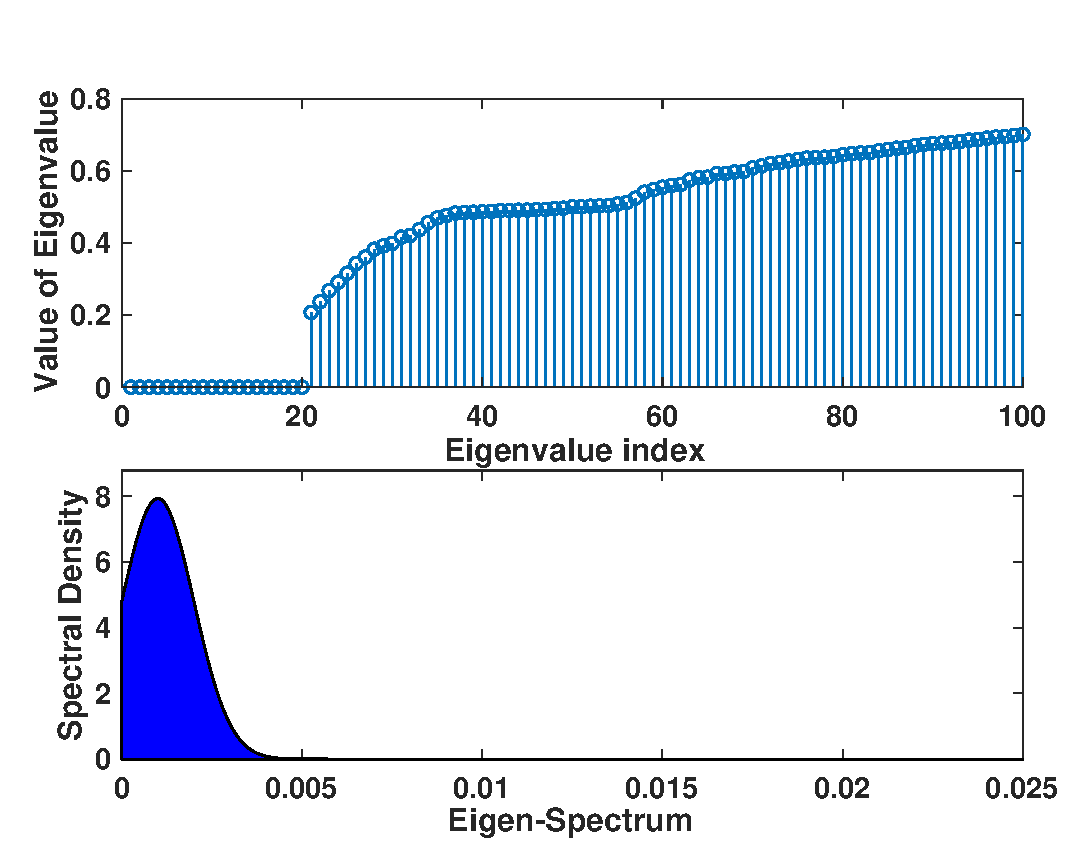
\includegraphics[trim=0.1cm 0cm 0.1cm 0.1cm, clip, width=1.0\linewidth]{Figures/EmailStemGraph}
	\caption{The smallest 100 Eigenvalues of the Email Dataset, with clear spectral gap along with the corresponding spectral density near the origin, showing a minimum at the value of the eigengap. The shaded area multiplied by the number of nodes $n$ predicts the number of clusters.}
	\label{fig:email}	
\end{figure} 

We display the process of spectral learning for both MaxEnt and Lanczos, by plotting the spectral density of both methods against the true eigenvalue spectral density in Figure \ref{fig:emaildensity}. In order to make a valid comparison, we smooth the implied density using a Gaussian kernel, with $\sigma = 10^{-3}$. We note that both MaxEnt and Lanczos approximate the ground truth better with a greater number of moments/steps $m$ and that Lanczos learns the extrema before the bulk of the distribution.

\begin{figure}[t]
	\centering
	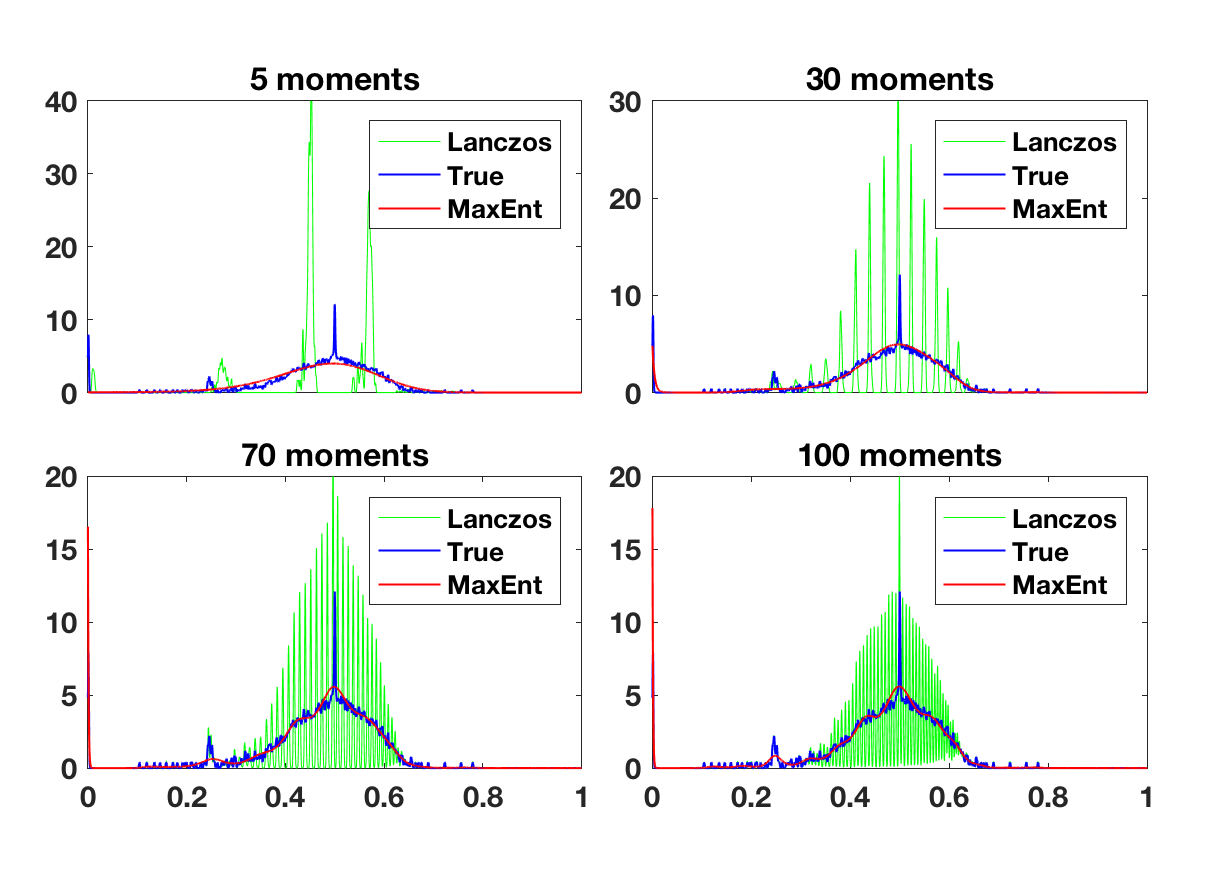
\includegraphics[trim=0.5cm 0.5cm 0.5cm 0.5cm, clip, width=1.0\linewidth]{Figures/Email_distribution}
	\caption{Spectral density for varying number of moments $m$, for both the MaxEnt and Lanczos algorithm as well as the ground truth.}
	\label{fig:emaildensity}	
\end{figure} 

We plot the log error against the number of moments for both MaxEnt and Lanczos in Figure \ref{fig:emailerror}, with MaxEnt showing superior performance.

\begin{figure}[t]
	\centering
	\begin{subfigure}{.5\linewidth}
		\centering
	\includegraphics[trim=0.2cm 0cm 1cm 0.5cm, clip, width=1.0\linewidth]{Figures/Error_for_Email}
\caption{Email Dataset}
\label{fig:emailerror}	
	\end{subfigure}%
	\begin{subfigure}{.5\linewidth}
		\centering
		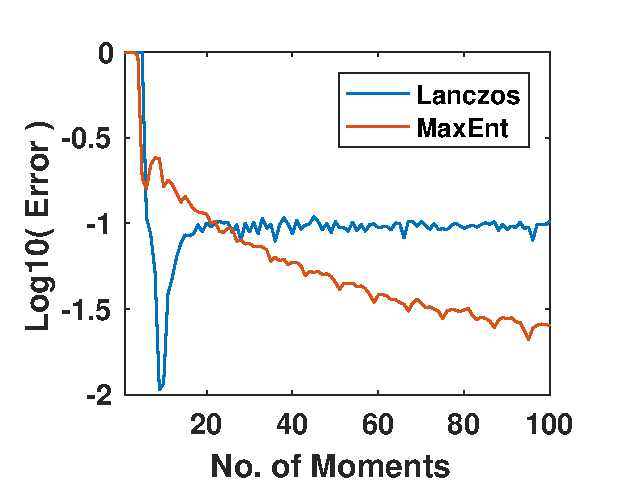
\includegraphics[trim=0.2cm 0cm 1cm 0.5cm, clip, width=1.0\linewidth]{Figures/Error_for_Netscience}
		\caption{NetScience Dataset}
		\label{fig:netscienceerror}
	\end{subfigure}
	\caption{Log error of community detection using MaxEnt and Lanczos algorithms on for differing number of moments $m$.}
	\label{fig:netscience}
\end{figure}

We repeat the experiment on the Net Science collaboration network, which represents a co-authorship network of $1,589$ scientists ($n = 1,589$) working on network theory and experiment \citep{newman2006finding}. The results in Figure \ref{fig:netscience} show that MaxEnt quickly outperforms the Lanczos algorithm after around $20$ moments.

\subsubsection{Large Real World Data}
For large datasets $n\gg10^{4}$, where the Cholesky decomposition becomes completely prohibitive even for powerful machines, we can no longer define a ground truth using a complete eigen-decomposition. We note that the ground truth supplied in \citep{mislove-2007-socialnetworks}, regarding each connected component in a group as a separate ground-truth community and removing communities with less than 3 nodes is not universal. This definition, along with that of self-declared group membership \citep{yang2015defining}, often leads to contradictions with our definition of a community, such as with the Orkut dataset, where the number of communities is greater than the number of nodes \citep{snapnets}. Beyond being impossible to learn such a value from the eigenspectra, if the main reason to learn about clusters is to partition groups and to summarise networks into smaller substructures, such a definition is undesireable.

We show that our method continues to faithfully approximate the spectra of large graphs, as shown in Figure \ref{fig:youtube150moments} by comparing with a kernel smoothed Lanczos approximation. We note that our spectrum displays Gibbs oscillations typical of MaxEnt, which in the case of a badly defined spectral gap (no clear spectral minimum), could lead to spurious minima.  
\begin{figure}	
	\centering
	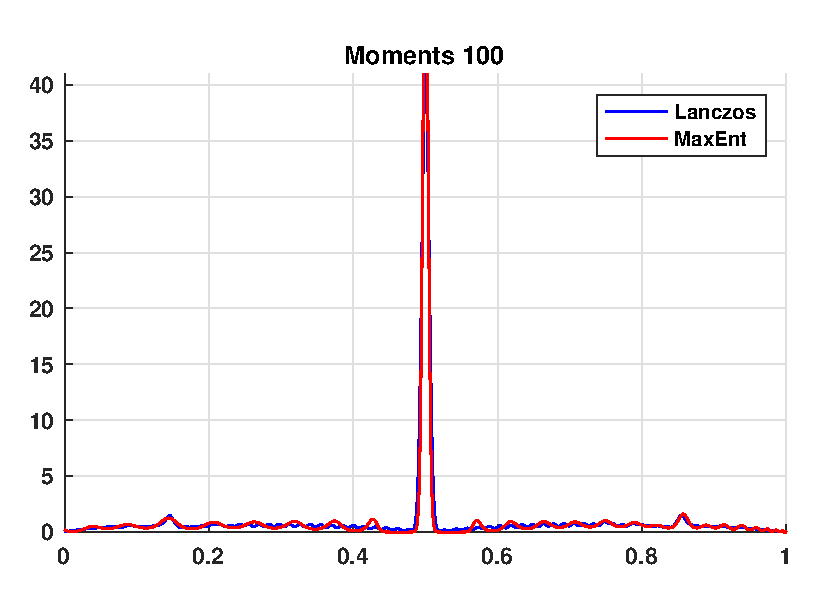
\includegraphics[trim=1.0cm 0.9cm 1cm 0.8cm, clip, width=1.0\linewidth]{Figures/YoutubeDistributionat150moments}
	\caption{Spectral Density for Youtube Dataset $m=150$, for MaxEnt and Lanczos Approximation}
	\label{fig:youtube150moments}	
\end{figure} 
We present our findings for the number of clusters in the DBLP ($n=317,080$), Amazon ($n=334,863$) and YouTube ($n=1,134,890$) networks \citep{snapnets} in Table \ref{table:largedata} for a varying number of moments. 

\begin{table}[t]
	\caption{Cluster rrediction by MaxEnt for DBLP ($n=317,080$), Amazon ($n=334,863$) and YouTube ($n=1,134,890$). }	\label{table:largedata}
	\begin{center}
		\begin{small}
			\begin{sc}
				\begin{tabular}{lcccr}
					\toprule
					Moments  & 40  & 70  & 100 \\
					\midrule
					DBLP    & $ 2.215\times 10^{4}$   & $8.468 \times 10^{3}$  & $8.313\times 10^{3}$   \\
					Amazon & $2.351\times 10^{4}$   & $1.146\times 10^{4}$   & $1.201\times 10^{4}$   \\
					Youtube & $4.023\times 10^{3}$   & $1.306\times 10^{4}$   & $1.900\times 10^{4}$   \\
					\bottomrule
				\end{tabular}
			\end{sc}
		\end{small}
	\end{center}
	\vskip -0.1in
\end{table}

\begin{table}[t]
	\caption{Average parameters estimated by MaxEnt for the 3 types of network }\label{learn_synnet_para}
	\begin{center}
		\begin{small}
			\begin{sc}
				\begin{tabular}{lcccr}
					\toprule
					$n$ & 50  & 100  & 150 \\
					%& $($p=0.6$)$ & $($p=0.4$)$ & ($m=0.4n$)\\
					\midrule
					Erdos-Renyi \\($p=0.6$)     & $0.600$   & $0.598$  & $ 0.6040$   \\
					Watts-Strogatz \\($p=0.4$)  & $0.4683$   & $0.4537$   & $0.4129$   \\
					Barabási-Albert  \\($r=0.4n$)   & $18.9360$ & $40.2389$  & $58.4275$   \\
					\bottomrule
				\end{tabular}
			\end{sc}
		\end{small}
	\end{center}
	\vskip -0.1in
\end{table}


\subsubsection{Learning Real-world Network Types using MaxEnt and Jensen-Shannon Divergence}
Determining which random graph models best fit real networks, characterised by their spectral divergence, so as to better understand their dynamics and characteristics has been explored in Biology \citep{takahashi2012discriminating}. We replicate their synthetic experiments using our approximate MaxEnt spectrum, with the results reported in Table \ref{learn_synnet_para}. 

We generate random graphs of a given size $n$ and parameters and then find its MaxEnt spectral characterisation. Then by generating other graphs of the same size, and running the Jensen-Shannon divergence between the original spectral density and the proposed through the inbuilt Python minimiser, we investigate whether one can recover the parameters of the input graph. We repeat the experiment for all 3 types of synthetic networks: Erdos-Renyi, Watts-Strogatz and Barabási-Albert, and for each type, we repeat for different network sizes $n = 50, 100, 150$. 

The results in Table \ref{learn_synnet_para} show that for randomly generated networks, given simply the approximate MaxEnt spectrum, we are able to rather well learn the parameters of the graph producing that spectrum. 

We also conduct another set of experiments to test our method for robustness against changing spectral properties with network scale. We generate a Barabási-Albert graph of $n=5000$ with given parameters and then try to minimise the divergence between random graphs of different types, free parameters and fixed nodal size $1000$. The results in Table \ref{table:learn_synnet_real_type} show that we successfully recover the correct type of the synthetic network. 

As a real word example, we look for which random net- work among Erdos-Renyi, Watts-Strogatz and Barbasi- Albert can best model the YouTube dataset. We do this by minimizing the divergence between YouTube Max-Ent spectral density and those of the randomly generated graphs. We find that the Barbasi-Albert gives the lowest divergence, which aligns with other findings for social networks \citep{barabasi1999emergence}.
\begin{table}[t]
	\caption{Minimum KL divergence between Entropic Spectrum of Youtube and that of Synthetic Networks}	\label{table:learn_synnet_real_type}
	\begin{center}
		\begin{small}
			\begin{sc}
				\begin{tabular}{lcccr}
					\toprule
					& Synthetic  & Youtube \\
					\midrule
					Erdos-Renyi  & $2.662$ &$7.728$\\
					Watts-Strogatz & $7.6123$ &$ 9.735$ \\
					Barabási-Albert & $\mathbf{2.001}$ & $ \mathbf{7.593} $\\
					\midrule
				\end{tabular}
			\end{sc}
		\end{small}
	\end{center}
	\vskip -0.1in
\end{table} 

%%%%%%%%%%%%%%%%%%%%%%%%%%%%%%%%%%%%%%%%%%%%%%%%%%%%%%%
%%%%%%%%%%%%%%%%%%%  Conclusion  %%%%%%%%%%%%%%%%%%%%%%%
%%%%%%%%%%%%%%%%%%%%%%%%%%%%%%%%%%%%%%%%%%%%%%%%%%%%%%%

\section{CONCLUSION}
We present an algorithm for learning the spectral density of large networks and propose a method for using the spectrum to learn the number of clusters within the network. We experimentally validate our approach on both synthetic and real world data. We further show that spectral divergence techniques can be faithfully reproduced using our approximative methods. 

The major advantage of the here presented algorithm using maximum entropy is its computational complexity which is $\mathcal{O}(n_{\mathrm{nz} } m d)$, where $n_\mathrm{nz}$ is the number of non-zeros of the matrix, $m$ is the number of moments we use and $d$ the number of random starting vectors. When compared to state-of-the-art algorithms using Lanczos iteration, our algorithm is seen to have smaller prediction errors compared to the ground truth.

As a byproduct, we present an alternative derivation of a bound on eigenvalue perturbations and relate this to the ratio of inter cluster to intra cluster links before the eigengap heuristic and thus our definition of communities breaks down. 


\bibliographystyle{abbrvnat}
\bibliography{bibi}

\end{document}
